\documentclass[landscape,final]{baposter}

\usepackage{times}
\usepackage{calc}
\usepackage{graphicx}
\usepackage{amsmath}
\usepackage{amssymb}
\usepackage{relsize}
\usepackage{multirow}
\usepackage{bm}

\usepackage{graphicx}
\usepackage{multicol}
\usepackage{ulem}

\usepackage{pgfbaselayers}
\pgfdeclarelayer{background}
\pgfdeclarelayer{foreground}
\pgfsetlayers{background,main,foreground}

\usepackage{helvet}
%\usepackage{bookman}
\usepackage{palatino}

\newcommand{\captionfont}{\footnotesize}

\selectcolormodel{cmyk}

\graphicspath{{template_images/}{images/}}

%%%%%%%%%%%%%%%%%%%%%%%%%%%%%%%%%%%%%%%%%%%%%%%%%%%%%%%%%%%%%%%%%%%%%%%%%%%%%%%%
%%%% Some math symbols used in the text
%%%%%%%%%%%%%%%%%%%%%%%%%%%%%%%%%%%%%%%%%%%%%%%%%%%%%%%%%%%%%%%%%%%%%%%%%%%%%%%%
% Format 
\newcommand{\Matrix}[1]{\begin{bmatrix} #1 \end{bmatrix}}
\newcommand{\Vector}[1]{\Matrix{#1}}
\newcommand*{\SET}[1]  {\ensuremath{\mathcal{#1}}}
\newcommand*{\MAT}[1]  {\ensuremath{\mathbf{#1}}}
\newcommand*{\VEC}[1]  {\ensuremath{\bm{#1}}}
\newcommand*{\CONST}[1]{\ensuremath{\mathit{#1}}}
\newcommand*{\norm}[1]{\mathopen\| #1 \mathclose\|}% use instead of $\|x\|$
\newcommand*{\abs}[1]{\mathopen| #1 \mathclose|}% use instead of $\|x\|$
\newcommand*{\absLR}[1]{\left| #1 \right|}% use instead of $\|x\|$

\def\norm#1{\mathopen\| #1 \mathclose\|}% use instead of $\|x\|$
\newcommand{\normLR}[1]{\left\| #1 \right\|}% use instead of $\|x\|$

\def\half{{\textstyle{1\over2}}}
\def\d{{\rm d}}
\font\dsrom=dsrom10
\def\one{\hbox{\dsrom 1}}

%%%%%%%%%%%%%%%%%%%%%%%%%%%%%%%%%%%%%%%%%%%%%%%%%%%%%%%%%%%%%%%%%%%%%%%%%%%%%%%%
% Multicol Settings
%%%%%%%%%%%%%%%%%%%%%%%%%%%%%%%%%%%%%%%%%%%%%%%%%%%%%%%%%%%%%%%%%%%%%%%%%%%%%%%%
\setlength{\columnsep}{0.7em}
\setlength{\columnseprule}{0mm}


%%%%%%%%%%%%%%%%%%%%%%%%%%%%%%%%%%%%%%%%%%%%%%%%%%%%%%%%%%%%%%%%%%%%%%%%%%%%%%%%
% Save space in lists. Use this after the opening of the list
%%%%%%%%%%%%%%%%%%%%%%%%%%%%%%%%%%%%%%%%%%%%%%%%%%%%%%%%%%%%%%%%%%%%%%%%%%%%%%%%
\newcommand{\compresslist}{%
\setlength{\itemsep}{1pt}%
\setlength{\parskip}{0pt}%
\setlength{\parsep}{0pt}%
}


%%%%%%%%%%%%%%%%%%%%%%%%%%%%%%%%%%%%%%%%%%%%%%%%%%%%%%%%%%%%%%%%%%%%%%%%%%%%%%
%%% Begin of Document
%%%%%%%%%%%%%%%%%%%%%%%%%%%%%%%%%%%%%%%%%%%%%%%%%%%%%%%%%%%%%%%%%%%%%%%%%%%%%%

\begin{document}

%%%%%%%%%%%%%%%%%%%%%%%%%%%%%%%%%%%%%%%%%%%%%%%%%%%%%%%%%%%%%%%%%%%%%%%%%%%%%%
%%% Here starts the poster
%%%---------------------------------------------------------------------------
%%% Format it to your taste with the options
%%%%%%%%%%%%%%%%%%%%%%%%%%%%%%%%%%%%%%%%%%%%%%%%%%%%%%%%%%%%%%%%%%%%%%%%%%%%%%
\typeout{Poster Starts}
\background{
  \begin{tikzpicture}[remember picture,overlay]%
    \draw (current page.north west)+(-2em,-0em) node[anchor=north west] {\hspace{-2em}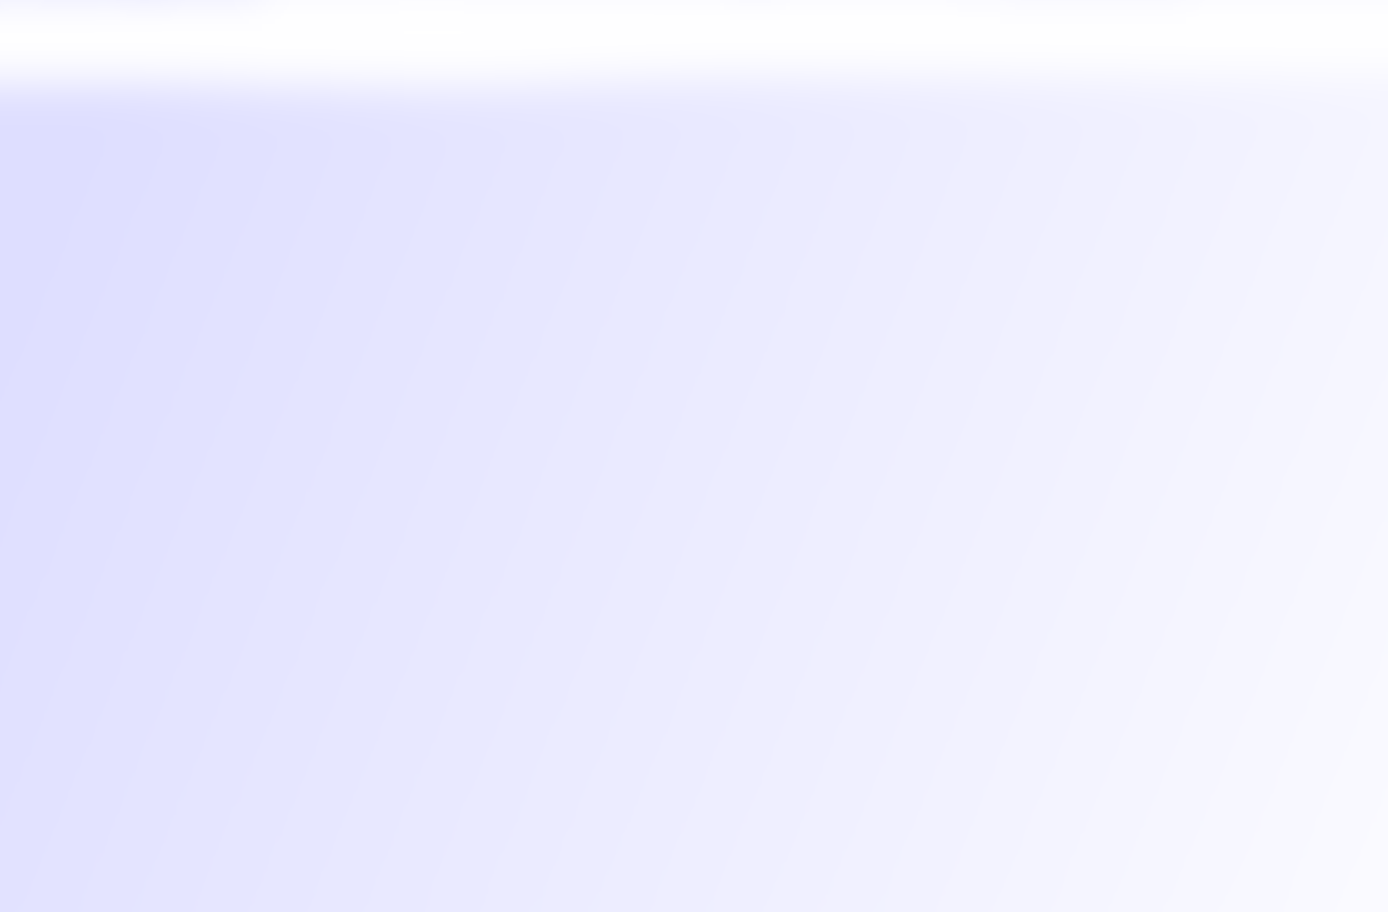
\includegraphics[height=1.1\textheight]{silhouettes_background}};
  \end{tikzpicture}%
}
\definecolor{silver}{cmyk}{0,0,0,0.3}
\definecolor{yellow}{cmyk}{0,0,0.9,0.0}
\definecolor{reddishyellow}{cmyk}{0,0.22,1.0,0.0}
\definecolor{black}{cmyk}{0,0,0.0,1.0}
\definecolor{darkYellow}{cmyk}{0,0,1.0,0.5}
\definecolor{darkSilver}{cmyk}{0,0,0,0.1}

\definecolor{lightyellow}{cmyk}{0,0,0.3,0.0}
\definecolor{lighteryellow}{cmyk}{0,0,0.1,0.0}
\definecolor{lighteryellow}{cmyk}{0,0,0.1,0.0}
\definecolor{lightestyellow}{cmyk}{0,0,0.05,0.0}
\begin{poster}{
  % Show grid to help with alignment
  grid=no,
  % Column spacing
  colspacing=1em,
  % Color style
  bgColorOne=lighteryellow,
  bgColorTwo=lightestyellow,
  borderColor=reddishyellow,
  headerColorOne=yellow,
  headerColorTwo=reddishyellow,
  headerFontColor=black,
  boxColorOne=lightyellow,
  boxColorTwo=lighteryellow,
  % Format of textbox
  textborder=roundedleft,
  % Format of text header
  eyecatcher=no,
  headerborder=open,
  headerheight=0.08\textheight,
  headershape=roundedright,
  headershade=plain,
  headerfont=\Large\textsf, %Sans Serif
  boxshade=plain,
%  background=shade-tb,
  background=plain,
  linewidth=2pt
  }
  % Eye Catcher
  {} % No eye catcher for this poster. If an eye catcher is present, the title is centered between eye-catcher and logo.
  % Title
  {\sf %Sans Serif
  %\bf% Serif
  High-Order, Adaptive Methods for Atomic Structure Calculations}
  % Authors
  {\sf %Sans Serif
  % Serif
  %Ond\v rej \v Cert\'\i k$^{1,2}$, John Pask$^1$, Pavel \v Sol\'\i n$^2$
  Ond\v rej \v Cert\'\i k$^{1,2}$, John Pask$^1$, Pavel Solin$^2$
  \hspace{3em}$^1$ Lawrence Livermore National Laboratory,
  $^2$ University of Nevada, Reno
  }
  % University logo
  {{\begin{minipage}{16em}
    \hfill
    
\includegraphics[height=5.5em]{llnl_logo}
  \end{minipage}}
  }

  \tikzstyle{light shaded}=[top color=baposterBGtwo!30!white,bottom color=baposterBGone!30!white,shading=axis,shading angle=30]

  % Width of left inset image
     \newlength{\leftimgwidth}
     \setlength{\leftimgwidth}{0.78em+8.0em}

%%%%%%%%%%%%%%%%%%%%%%%%%%%%%%%%%%%%%%%%%%%%%%%%%%%%%%%%%%%%%%%%%%%%%%%%%%%%%%
%%% Now define the boxes that make up the poster
%%%---------------------------------------------------------------------------
%%% Each box has a name and can be placed absolutely or relatively.
%%% The only inconvenience is that you can only specify a relative position 
%%% towards an already declared box. So if you have a box attached to the 
%%% bottom, one to the top and a third one which should be in between, you 
%%% have to specify the top and bottom boxes before you specify the middle 
%%% box.
%%%%%%%%%%%%%%%%%%%%%%%%%%%%%%%%%%%%%%%%%%%%%%%%%%%%%%%%%%%%%%%%%%%%%%%%%%%%%%
    %
    % A coloured circle useful as a bullet with an adjustably strong filling
    \newcommand{\colouredcircle}[1]{%
      \tikz{\useasboundingbox (-0.2em,-0.32em) rectangle(0.2em,0.32em); \draw[draw=black,fill=baposterBGone!80!black!#1!white,line width=0.03em] (0,0) circle(0.18em);}}

%%%%%%%%%%%%%%%%%%%%%%%%%%%%%%%%%%%%%%%%%%%%%%%%%%%%%%%%%%%%%%%%%%%%%%%%%%%%%%
  \headerbox{Abstract}{name=contribution,column=0,row=0}{
%%%%%%%%%%%%%%%%%%%%%%%%%%%%%%%%%%%%%%%%%%%%%%%%%%%%%%%%%%%%%%%%%%%%%%%%%%%%%%
   We compare several high-order methods for solving the radial Schr\"odinger
   and Dirac equations, in particular, spectral finite element method, $p$-FEM,
   $h$-FEM, and $hp$-FEM. All methods provide a robust way of calculating all
   eigenstates to machine precision. They differ in the rate of convergence and
   whether a good initial mesh is needed or not, as well as providing robust
   error control.
 }

%%%%%%%%%%%%%%%%%%%%%%%%%%%%%%%%%%%%%%%%%%%%%%%%%%%%%%%%%%%%%%%%%%%%%%%%%%%%%%
  \headerbox{Motivation}{name=motivation,column=0,below=contribution}{
%%%%%%%%%%%%%%%%%%%%%%%%%%%%%%%%%%%%%%%%%%%%%%%%%%%%%%%%%%%%%%%%%%%%%%%%%%%%%%
The need for an efficient solution to the radial Dirac equation arises
in the calculation of the equation of state and opacity of materials
under extreme conditions.

These calculations often rely on
self-consistent average-atom codes to compute the atomic structure for a
representative atom in a plasma. For plasmas at low densities and high
temperatures, a very large number of Rydberg states are accessible,
often requiring the calculation of principal quantum numbers of 100 or
higher.

This poses a challenge for the existing average-atom models,
since they have difficultly in resolving all the bound states just below
the continuum, and accurately computing the wave-function of
high-principal-quantum-number states near the nucleus.
  }

%%%%%%%%%%%%%%%%%%%%%%%%%%%%%%%%%%%%%%%%%%%%%%%%%%%%%%%%%%%%%%%%%%%%%%%%%%%%%%
\headerbox{Higher-Order FE Methods}{name=hpfem,column=0,below=motivation,span=1,above=bottom}{
%%%%%%%%%%%%%%%%%%%%%%%%%%%%%%%%%%%%%%%%%%%%%%%%%%%%%%%%%%%%%%%%%%%%%%%%%%%%%%
\small
Finite element (FE) methods\cite{solin} partition the problem domain into
subdomains called "elements", and represent the desired solution as a linear
combination of piecewise polynomials defined within each element; wherein $h$
characterizes the element size and $p$, the polynomial order.
\begin{itemize}
\item $h$-FEM increases accuracy by decreasing $h$
\item $p$-FEM increases accuracy by increasing $p$
\item $hp$-FEM increases accuracy by refining both $h$ and $p$ simultaneously
\end{itemize}
Basis is polynomial and strictly local $\to$ robust and naturally parallel
method for the solution of large-scale PDE problems, as in electronic
structure\cite{pask}.

%Plane waves (PW) are pseudospectral method, on the same level as spectral
%element method (uniform-$p$-FEM), which is a subset of $p$-FEM, which is a
%subset of $hp$-FEM.

$hp$-FEM has many favorable properties: exponential convergence, automatic
adaptivity (no a priori knowledge needed), any geometry and boundary
conditions, and systematic error control.
  }

%%%%%%%%%%%%%%%%%%%%%%%%%%%%%%%%%%%%%%%%%%%%%%%%%%%%%%%%%%%%%%%%%%%%%%%%%%%%%%
\headerbox{Schr\"odinger Equation}{name=schroed,column=1}{
%%%%%%%%%%%%%%%%%%%%%%%%%%%%%%%%%%%%%%%%%%%%%%%%%%%%%%%%%%%%%%%%%%%%%%%%%%%%%%
Radial Schr\"odinger equation:
$$(-\half \rho^2 R')' + (\rho^2 V + \half l(l+1)) R = \epsilon \rho^2 R$$
Weak formulation
$$
\int \half \rho^2 R'v' + (\rho^2 V + \half l(l+1)) Rv \d\rho
        -\half[\rho^2R'v]_0^a =
$$
$$
= \epsilon \int \rho^2 Rv \d\rho
$$
Discretization in an FE basis produces a generalized eigenvalue problem
of the form $A x = \lambda B x$.

Setting boundary term $\half[\rho^2R'(\rho)v(\rho)]_0^a=0$ imposes $R'(a)=0$
but no restriction on $R$ at $\rho=0$, due to vanishing of $\rho^2$. We impose
$R(a)=0$ by restricting the FE basis and allow the natural BC at $\rho=0$: we
solve for $R(0)$ directly (note that in general $R(0)\neq 0$).
}

%%%%%%%%%%%%%%%%%%%%%%%%%%%%%%%%%%%%%%%%%%%%%%%%%%%%%%%%%%%%%%%%%%%%%%%%%%%%%%
  \headerbox{Dirac Equation}{name=dirac,column=1,below=schroed,row=0}{
%%%%%%%%%%%%%%%%%%%%%%%%%%%%%%%%%%%%%%%%%%%%%%%%%%%%%%%%%%%%%%%%%%%%%%%%%%%%%%
Radial Dirac equations:
$$
-\hbar c \left({\d\over\d\rho} - {\kappa\over\rho}\right)Q + (V+mc^2-W)P=0
$$

$$
+\hbar c \left({\d\over\d\rho} + {\kappa\over\rho}\right)P + (V-mc^2-W)Q=0
$$
weak formulation:
$$
\int PVv_1 \d\rho -\hbar c Q'v_1 + \hbar c{\kappa\over\rho}Qv_1 \d\rho =
\epsilon \int Pv_1 \d\rho
$$
$$
\int \hbar c P'v_2 + \hbar c{\kappa\over\rho}Pv_2 + (V -2mc^2)Qv_2 \d\rho =
\epsilon \int Q v_2 \d\rho
$$
Correspondence between the radial Schr\"odinger and Dirac equation is:
$$
\rho^2 R^2(\rho) = P^2(\rho) + Q^2(\rho)
$$
  }
%%%%%%%%%%%%%%%%%%%%%%%%%%%%%%%%%%%%%%%%%%%%%%%%%%%%%%%%%%%%%%%%%%%%%%%%%%%%%%
\headerbox{References}{name=references,column=1,above=bottom,below=dirac}{
%%%%%%%%%%%%%%%%%%%%%%%%%%%%%%%%%%%%%%%%%%%%%%%%%%%%%%%%%%%%%%%%%%%%%%%%%%%%%%
    \tiny
    %\smaller
    \vspace{-0.4em}
    \bibliographystyle{ieee}
    \renewcommand{\section}[2]{\vskip 0.05em}
      \begin{thebibliography}{1}\itemsep=-0.01em
      \setlength{\baselineskip}{0.4em}
      \bibitem{romanowski}
        Z. Romanowski
        \newblock Application of h-adaptive, high order finite element method
        to solve radial Schr\"odinger equation
        \newblock {\em  Molecular Physics (2009)}
      \bibitem{solin}
      P. Solin, K. Segeth, I Dolezel
        \newblock Higher-Order Finite Element methods
        \newblock {\em Chapman \& Hall/CRC Press (July 2003)}
      \bibitem{pask}
      J.E. Pask and P.A. Sterne
        \newblock Finite element methods in ab initio electronic structure
        calculations
        \newblock {\em Modelling Simul. Mater. Sci. Eng. 13, R71
      (2005)}
      \end{thebibliography}
  }%
%%%%%%%%%%%%%%%%%%%%%%%%%%%%%%%%%%%%%%%%%%%%%%%%%%%%%%%%%%%%%%%%%%%%%%%%%%%%%%
  \headerbox{Hydrogen Atom (3 lowest states of Schr\"odinger equation for $Z=1$)}{name=hydrogen,column=2,span=2,row=0}{
%%%%%%%%%%%%%%%%%%%%%%%%%%%%%%%%%%%%%%%%%%%%%%%%%%%%%%%%%%%%%%%%%%%%%%%%%%%%%%
Comparison of uniform-$p$-FEM, $h$-FEM (Romanowski\cite{romanowski}),
$p$-FEM (two different meshes) and $hp$-FEM:\\
    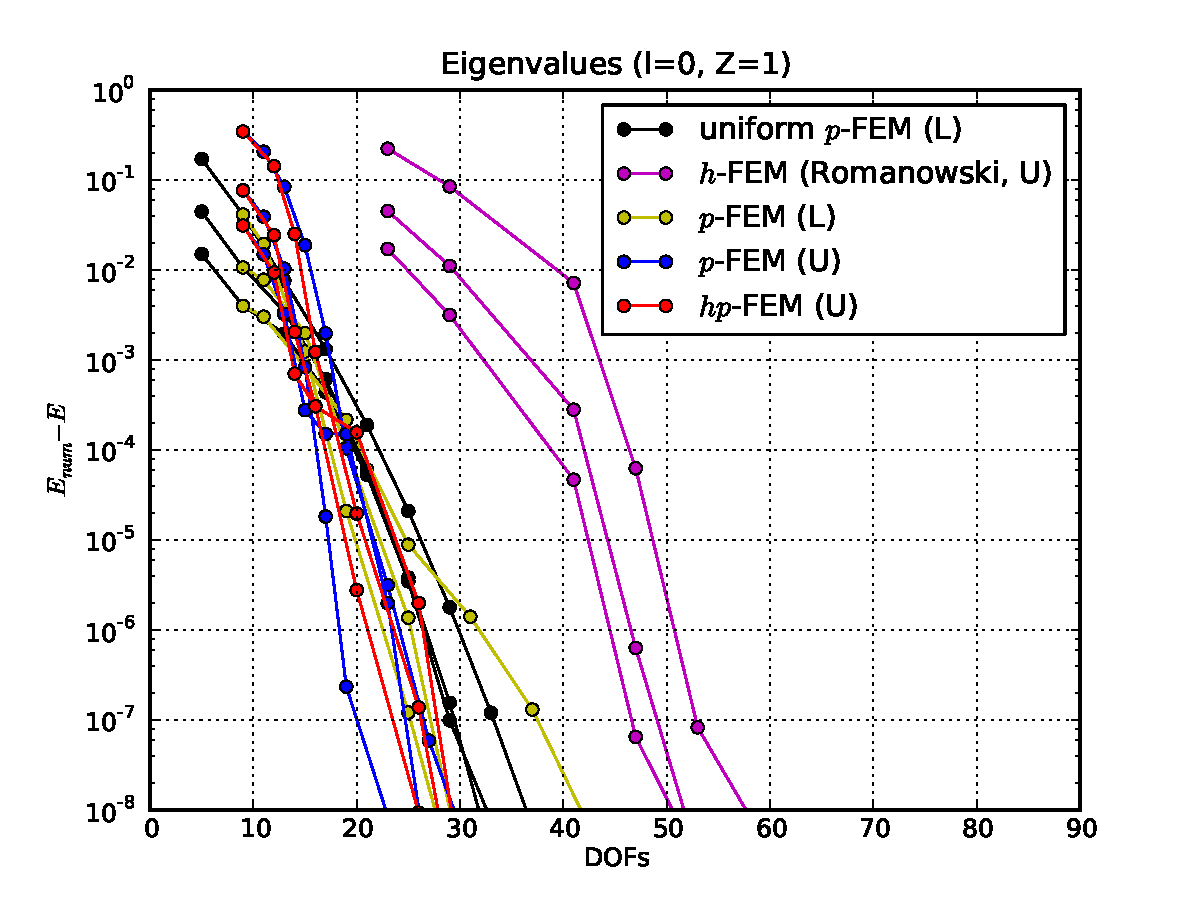
\includegraphics[height=0.25\textheight]{hydrogen_l_0}
    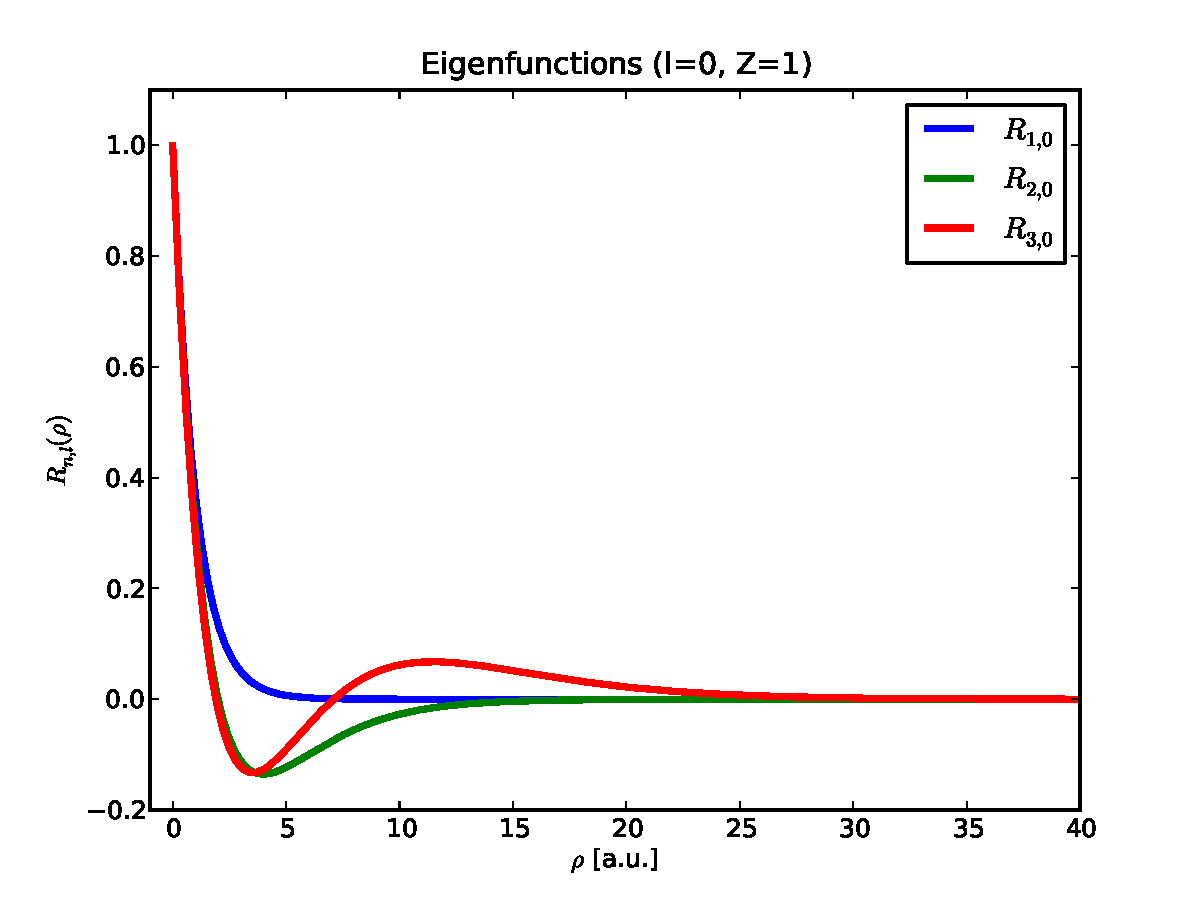
\includegraphics[height=0.25\textheight]{hydrogen_vec}\\
\smaller
(L) starts from logarithmic initial mesh, (U) starts from uniform initial mesh.
Domain is $[0, 100]$ (much bigger than shown in Figs).
  }%
%%%%%%%%%%%%%%%%%%%%%%%%%%%%%%%%%%%%%%%%%%%%%%%%%%%%%%%%%%%%%%%%%%%%%%%%%%%%%%
  \headerbox{Silver Atom (50 lowest states of Schr\"odinger equation for $Z=47$)}{name=silver,column=2,span=2,below=hydrogen}{
%%%%%%%%%%%%%%%%%%%%%%%%%%%%%%%%%%%%%%%%%%%%%%%%%%%%%%%%%%%%%%%%%%%%%%%%%%%%%%
Comparison of uniform-$p$-FEM (two different meshes), $p$-FEM and $hp$-FEM
(domain $[0, 150]$):\\
    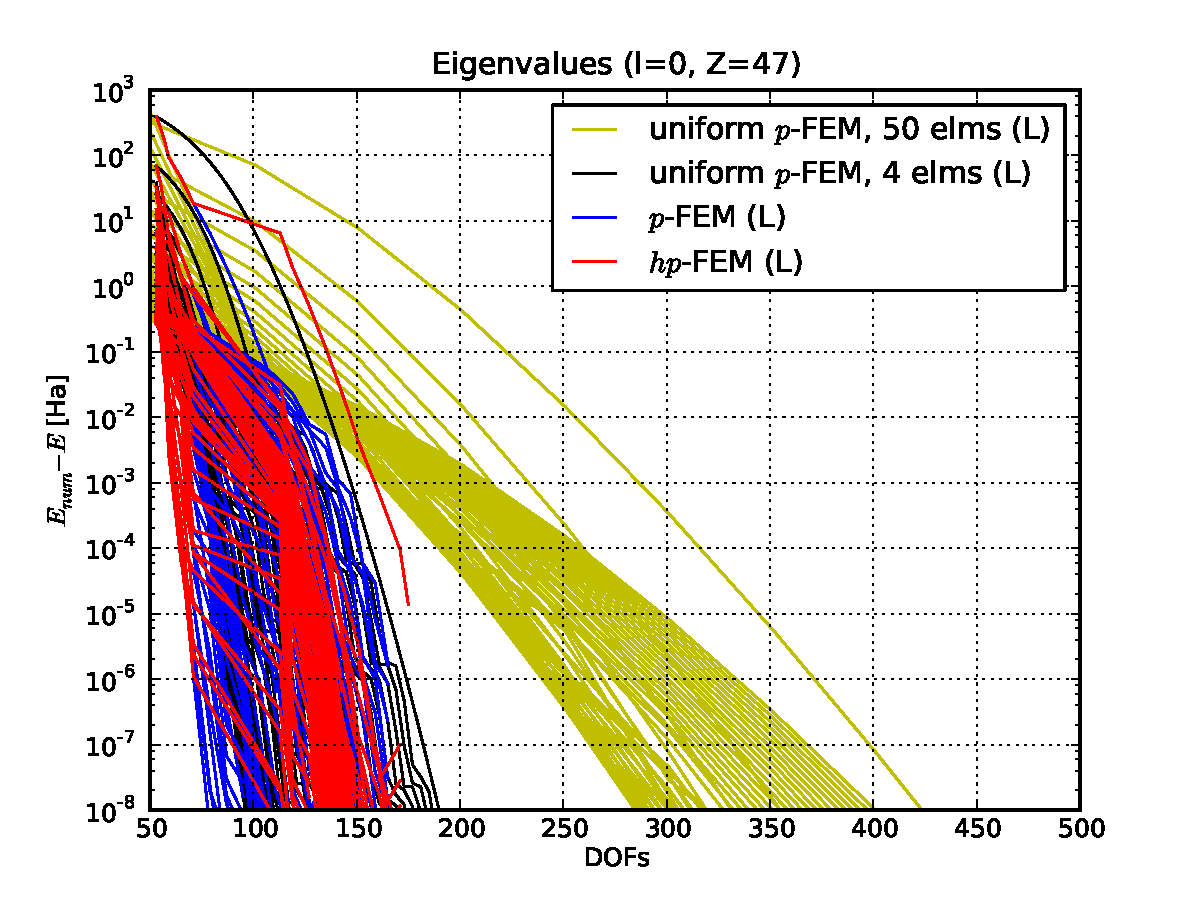
\includegraphics[height=0.25\textheight]{silver_l_0}
    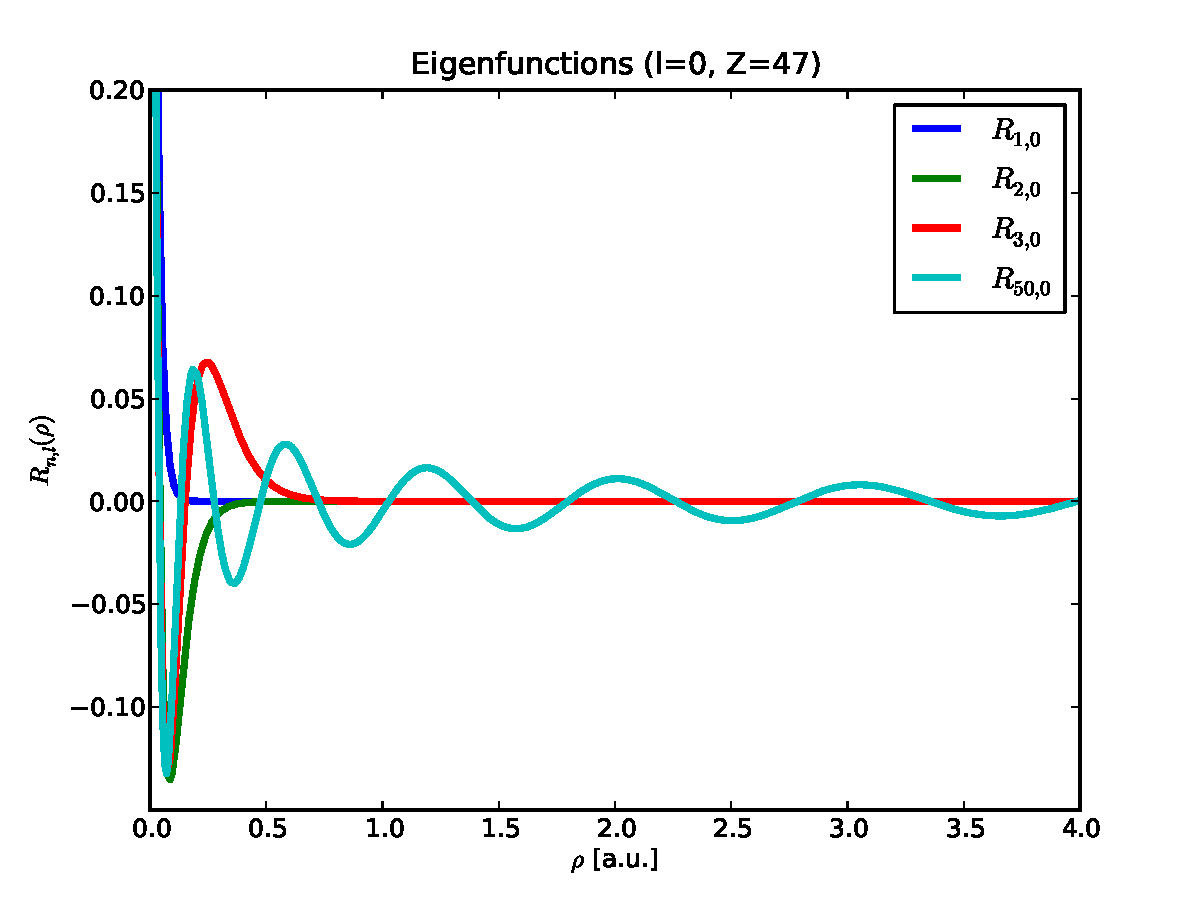
\includegraphics[height=0.25\textheight]{silver_vec}
  }%
%%%%%%%%%%%%%%%%%%%%%%%%%%%%%%%%%%%%%%%%%%%%%%%%%%%%%%%%%%%%%%%%%%%%%%%%%%%%%%
\headerbox{Conclusions}{name=conclusions,column=2,span=1,below=silver,above=bottom}{
%%%%%%%%%%%%%%%%%%%%%%%%%%%%%%%%%%%%%%%%%%%%%%%%%%%%%%%%%%%%%%%%%%%%%%%%%%%%%%
\smaller
High-order adaptive FE methods provide a robust, variational alternative to
conventional shooting methods, finding all desired states simultaneously, with
accuracy and orthogonality approaching machine precision.

High-order $p$-FEM and $hp$-FEM are superior to $h$-FEM in atomic structure
context.

$hp$-FEM is the method of choice when little or no a priori information is
available; however, in atomic-structure context, much is known --> high-order
$p$-FEM can be superior in practice (due to practical constraints on $hp$-FEM
mesh --- further research is needed).

Future: extend present Schroedinger formulations to Dirac equation and
self-consistent calculations.
  }%
%%%%%%%%%%%%%%%%%%%%%%%%%%%%%%%%%%%%%%%%%%%%%%%%%%%%%%%%%%%%%%%%%%%%%%%%%%%%%%
  \headerbox{Acknowledgment}{name=acknowledgment,column=3,span=1,above=bottom}{
%%%%%%%%%%%%%%%%%%%%%%%%%%%%%%%%%%%%%%%%%%%%%%%%%%%%%%%%%%%%%%%%%%%%%%%%%%%%%%
  \smaller
Calculated using Hermes1D (hp-FEM group at UNR:
\texttt{http://hpfem.org/}) and sle1d
(J.E. Pask, LLNL).

   This work performed under the auspices of the U.S. Department of Energy by
   Lawrence Livermore National Laboratory under Contract DE-AC52-07NA27344.
  }%
%%%%%%%%%%%%%%%%%%%%%%%%%%%%%%%%%%%%%%%%%%%%%%%%%%%%%%%%%%%%%%%%%%%%%%%%%%%%%%
  \headerbox{Meshes}{name=meshes,column=3,span=1,below=silver,above=acknowledgment}{
%%%%%%%%%%%%%%%%%%%%%%%%%%%%%%%%%%%%%%%%%%%%%%%%%%%%%%%%%%%%%%%%%%%%%%%%%%%%%%
  \smaller
  }%
\end{poster}%
%
\end{document}
